\chapter{\nmu Metodologia} % (fold)
\label{cha:metodologia}

% Etapas em que o trabalho foi realizado
% 	levantamento bibliografico
% 	codificação
% 	testes
% 	levantamento de algoritmos
% 	ferramentas utilizadas
% 	justificativa das escolha dos metodos/algoritmos
% escolha dos pacotes para teste

\section{Levantamento bibliográfico} % (fold)
\label{sec:levantamento_bibliogr_fico}

Com o auxilio de ambientes como o Periódicos Capes, \textit{ebrary} e Google Acadêmico, foi levantado estudos em \textit{string matching} que pudessem vir a ser interessantes para a ordenação dos candidatos.  Por ser uma área estudada ate mesmo antes da modernização e popularização de computadores sejam por fins militares ou puramente científicos, este foi um dos pontos de difícil escolha de métodos devido a vasta diversidade da qual se é possível encontrar. Guiados por estudos recentes como o de Xu \cite{xu2013bit} com processamento usando GPUs ou mais antigos como o de Galil \cite{galil1988data}, um dos nomes que normalmente eram citados era o de Levenshtein e seu trabalho de 1966 \cite{levenshtein1966}. Este algoritmo por si só apontou outras duas alternativas, sendo uma delas uma variação do primeiro para maior exatidão de resultados. Assim, o levantamento indicava três algoritmos como candidatos para a solução do trabalho proposto. O algoritmo de \textit{Smith-Waterman}, a distância de \textit{Levenshtein} e sua variação na distância de \textit{Damerau-Levenshtein}.

% section levantamento_bibliogr_fico (end)


\section{Ferramentas} % (fold)
\label{sec:codifica_o}

Observado a necessidade de métodos que apresentassem resultados mais intuitivos ao usuário, duas escolhas deviam ser tomadas para objetividade do estudo: a escolha da plataforma e gerenciador a adotado para base do estudo e qual linguagem seria adotada para o trabalho.

Dentre os grandes grupos que a comunidade Linux se divide, distribuições oriundas do \textit{Debian} e do \textit{Slackware} são as predominantes. Dentre estas duas e suas ramificações, o Ubuntu é uma das distribuições mais indicadas e adotadas por pessoas que estão adentrando no mundo Linux. Desta forma o \textit{APT} torna-se o candidato escolhido dentro o grupo de gerenciadores de repositórios de pacotes. Como distribuição adotada então para desenvolvimento e teste no estudo, foi adotada o Ubuntu 14.04. 

Para uma agilização na obtenção de resultados para os objetivos, foi adotada a linguagem \textit{Python} por apresentar uma interface de interação com o gerenciador de pacote escolhido para uso neste trabalho, \nameref{subs:apt} e por ser de fácil prototipagem de código ao proporcionar um rápido e enxuto desenvolvimento de código. Para a edição de texto foi utilizado o \textit{Sublime-Text 2} com plugins do \textit{pylint} e \textit{PEP8} na tentativa de manter a padronização de código, documentação, coesão e coerência do protótipo.

Como forma de controle do tempo e no intuito de manter o desenvolvimento mais proximo do planejado, foi utilizado o \href{https://trello.com}{Trello} para lanças as atividade e definir as datas limites para entregas, fazendo com que a metodologia aproximasse à programação extrema (eXtreme Programming) ao apresentar contextos como fases pequenas (uma ou duas semanas), \textit{design} simples, padronização e refatoração de código.


%\section{Codificação} % (fold)
%\label{sec:codifica_o}


% section codifica_o (end)

\section{Algoritmos Propostos} % (fold)
\label{sec:algoritmos_propostos}

O interesse no estudo seja apresentar alternativas para o modelo de busca apresentado hoje no gerenciador e não novos algoritmos de aproximação de \textit{string}, foram priorizados algoritmos de implementação pouco rebuscada, que apresentassem bons resultados de ordenação de \textit{strings} e que já estivessem implementados em linguagem \textit{Python}. Desta forma, foram escolhidos três algoritmos disponibilizados no \href{https://pypi.python.org/}{PyPI}. São eles:

\begin{itemize}
	\item \href{https://pypi.python.org/pypi/swalign/}{swalign}\\
	Pacote que oferece o algoritmo de ordenação de \textit{Smith-Waterman}. Utilizada a versão $0.3.1$.
	\item \href{https://pypi.python.org/pypi/python-Levenshtein/}{python-Levenshtein}\\
	Pacote que oferece o algoritmo de ordenação de \textit{Levenshtein}.Utilizada a versão $0.11.2$.
	\item \href{https://pypi.python.org/pypi/pyxDamerauLevenshtein/}{pyxDamerauLevenshtein}\\
	Pacote que oferece o algoritmo de ordenação de \textit{Damerau-Levenshtein}. Utilizada a versão $1.2$.
\end{itemize}

Também foi utilizado o algoritmo de \textit{match} exato, o qual se idealiza na necessidade de ter a \textit{string} procurada presente no nome do pacote. Esta busca já é implementada no processo de \textit{search} do APT, porém ela aparece em segundo patamar de ordenação. Assim, foi implementado também um método de ordenação baseada apenas no \textit{match} exato  da \textit{string} de entrada pelo nome do pacote.


\section{Execução dos experimentos}

Definido os algoritmos que seriam utilizados no estudo, iniciou-se então a fase de prototipagem de código. O primeiro passo foi a familiarização com o pacote {\code apt}, disponibilizado por padrão na instalação do {\code python2.7} nas distribuições \textit{Debian-like}. Este pacote possibilita a busca, instalação e remoção de pacotes. Para tal foi utilizada a classe {\code apt.cache.Cache} que nos possibilita verificar a existência de um pacote na lista de candidatos por meio da interface {\code \_\_getitem\_\_} padrão do \textit{Python}. O \autoref{proto_apt} apresenta a versão final deste protótipo, onde se era testado por padrão no método a procura e instalação do pacote {\code git} enquanto na rotina principal se testava as mesmas rotinas para o inexistente pacote {\code gito}.



O estudo deste pacote possibilitou a a evolução de um esqueleto de código que permitiria o teste dos distintos algoritmos de \textit{string-matching}. O primeiro a ser escrito foi o de \textit{match} exato, apresentado no \autoref{proto_exact}. Este esqueleto oferecia elementos básicos aos prototipos que seriam criados a seguir, são eles:

\begin{description}
	\item[Classe Pack] Classe básica construída para armazenar os resultados obtidos dos algoritmos e posteriormente ordena-los. É formada basicamente pelo método de formatação de impressão do pacote, o nome do pacote, o \textit{ratio} do pacote (usado para classificação) e os métodos que podem vir a ser utilizados pelas rotinas de ordenação de listas.
	\item [\_parser] Objeto responsável por realizar o \textit{parser} das aplicações, oferecendo \textit{flags} de controle, como quantidade máxima a ser listada no resultado, \textit{ratio} mínimo a ser impresso, inclusão de prefixos e sufixos comuns ao nome do pacote procurado para classificação e a opção de executar um \textit{pool} de \textit{threads} na rotina a fim de agiliza-la. Esta última opção foi classificada como depreciada devido a instabilidade que gerava no momento de ordenação dos pacotes.
\end{description}


Este modelo foi fundamental para a escrita dos outros três protótipos deste trabalho, apresentados em \autoref{proto_leven}, \autoref{proto_damerau} e \autoref{proto_smith} no \autoref{anexos} deste documento. Como a estrutura do protótipo era mantida para os demais algoritmos, o único momento de retrabalho foi com o algoritmo de \textit{Smith-Waterman}, onde o pacote retornava uma lista de valores que deviam ser classificados, o que  necessitou a reescrita de um método de ordenação dos pacotes, já que para este algoritmo oferecido pelo pacote em especial não havia um retorno de uma simples distância ou \textit{ratio} de aproximação.


Para a obtenção dos resultados, foi utilizado um {\code Core™ i7 CPU 870} (\textit{2.93GHz})  e $3.8GB$ de RAM rodando sistema Ubuntu 14.04 LTS 64-bits. Os comandos foram todos executados em primeiro plano sem outra aplicação rodando em conjunto e foram-se efetuados cinco medidas consecutivas do tempo e retirada a média entre elas. A medida de tempo foi obtida executando a chamada das aplicações precedidas do comando {\code time} e tomado como resultado o valor retornado para o usuário. Na \autoref{fig:figuras_xpto} é possível observar um exemplo da procura pelo pacote \textit{xpto} no {\code apt}. Neste exemplo, o valor que seria considerado seria o de $890$ ms.

\begin{figure}[htbp]
  \centering
	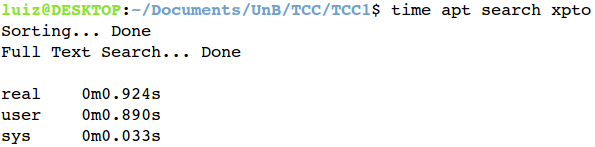
\includegraphics[width=0.8\textwidth]{figuras/xpto}
  \caption{Exemplo do uso do comando {\code time}}
  \label{fig:figuras_xpto}
\end{figure}

\section{Funcionalidades descartadas}

Também foi implementada a possibilidade de uso do padrão \textit{thread pool} para agilizar os resultados. Todavia, foi encontrada a dificuldade em manter a ordenação das listas, fazendo com que a opção fosse descontinuada ate segundo momento, porém não totalmente descartada, visto que em alguns testes houve redução de aproximadamente um terço do tempo gasto sem o uso de \textit{threads}. 
